\chapter{PGF}
\label{sec:pgf}

PGF和Beamer的作者都是Till Tantau (1975--)\indexTantau{} \footnote{柏林工业大学1999年电脑学士,2001年数学学士,2003年电脑博士。2004年伯克利访问学者,2005年吕贝克大学 (University of Lübeck) 理论计算机研究所教授。}。Tantau当初开发Beamer是为了准备2003年他的博士学位论文答辩,之后它在CTAN上流行开来。2005年PGF从Beamer项目中分离出来,成为一个独立的宏包\citep{Tantau_2010}。

\section{准备工作}

一般人们并不直接使用PGF底层命令,而是通过它前端TikZ来调用。在引用 \texttt{tikz} 宏包之前,用户需要设置PGF系统驱动。比如 \texttt{dvipdfmx} 的设置方法如下,使用 \texttt{pdflatex} 和 \texttt{xelatex} 时,它知道驱动是谁。

\begin{Code}[]
\def\pgfsysdriver{pgfsys-dvipdfmx.def}
\usepackage{tikz}
\end{Code}

PGF的缺省长度单位是1cm,我们也可以改用其它单位。注意这样预定义的长度单位有时会失效,这可能是PGF的bug。

\begin{Code}[]
\pgfsetxvec{\pgfpoint{10pt}{0}}
\pgfsetyvec{\pgfpoint{0}{10pt}}
\end{Code}

TikZ提供 \verb|\tikz| 命令和 \texttt{tikzpicture} 环境,具体绘图指令可以放在 \verb|\tikz| 后面,也可以放在 \texttt{tikzpicture} 中间。两者效果相同,用户可以任意选择。为了节省空间,本节的示例将省略部分环境代码。

\begin{Code}[]
\tikz ...   %绘图命令
\begin{tikzpicture}
...         %绘图命令
\end{tikzpicture}
\end{Code}

\ref{sec:pst_setup} 小节提到,为了节省编译时间,我们可以用 \texttt{preview} 宏包生成独立的图形文件。对于PGF我们也可以如法炮制,虽然这样做不是必须的。

\begin{example}[h]
\begin{Code}[]
\documentclass{article}
\usepackage[active,tightpage,xetex]{preview}
\usepackage{tikz}

\begin{document}
\begin{preview}
\begin{tikzpicture}
...
\end{tikzpicture}
\end{preview}
\end{document}
\end{Code}
\caption{制作独立的PGF图形文件}
\label{exa:pgf}
\end{example}

\section{基本图形对象}
\subsection{直线和矩形}

PGF绘图命令的语法和\MP{}有点类似。在 \autoref{exa:pgf_line} 中,\verb|\draw| 称为一个命令,它后面的 \texttt{--}、 \texttt{cycle}、 \texttt{rectangle} 等称为操作,\texttt{[rounded corners]} 称作一个选项。\texttt{--} 用来画直线,\texttt{rectangle} 画矩形; \texttt{cycle} 用来封闭路径,前两个三角形看起来一样,其实只有第二个才是真正的封闭路径;\texttt{[rounded corners]} 用来给图形加圆角。

操作都需要一个起始点参数,比如第一行代码第一个 \texttt{--} 操作的起始点是(0,0);第二行 \texttt{cycle} 的起始点是(7,2);第四行 \texttt{rectangle} 的起始点是(15,0),也就是矩形的一个顶点,(19,2)是其对角顶点。

\begin{example}[h]
\begin{FBTDemo}[numbers=left]{\includegraphics[page=4]{pgf.pdf}}
\draw (0,0)--(4,0)--(2,2)--(0,0);
\draw (5,0)--(9,0)--(7,2)--cycle;
\draw [rounded corners] (10,0)--(14,0)--(12,2)--cycle;
\draw (15,0) rectangle (19,2);
\draw [rounded corners] (20,0) rectangle (24,2);
\end{FBTDemo}
\caption{PGF 直线和矩形}
\label{exa:pgf_line}
\end{example}

\subsection{圆、椭圆、弧}

圆、椭圆、弧等形状的画法如下。圆的参数是圆心和半径,椭圆的参数是中心、长径、短径。圆弧的参数是起始点,起始角度、终止角度、半径;椭圆弧则把半径换成了长径和短径。

\begin{example}[h]
\begin{FBTDemo}[]{\includegraphics[page=5]{pgf.pdf}}
\draw (1,1) circle (1);
\draw (5,1) ellipse (2 and 1);
\draw (10,1) arc (0:270:1);
\draw (15,1) arc (0:270:2 and 1);
\end{FBTDemo}
\caption{PGF 圆、椭圆、弧}
\label{exa:pgf_circle}
\end{example}

\vspace{-10pt}
\subsection{曲线}

我们把直线的 \texttt{--} 换成 \texttt{..},就得到贝塞尔曲线,它需要至少一个控制点 (\autoref{exa:pgf_curve} 第一行) 。抛物线用 \texttt{parabola},代码第六行的(5,1)是它的起始点,(7.414,2)是终止点,\texttt{bend (6,0)}指定了顶点。

\begin{example}[h]
\begin{FBTDemo}[numbers=left]{\includegraphics[page=6]{pgf.pdf}}
\draw (0,0)..controls (2,2) and (4,2)..(4,0);
\filldraw (0,0) circle (.1)
    (2,2) circle (.1)
    (4,2) circle (.1)
    (4,0) circle (.1);
\draw (5,1) parabola bend (6,0) (7.414,2);
\filldraw (5,1) circle (.1)
    (6,0) circle (.1)
    (7.414,2) circle (.1);
\draw (8,0) sin (10,2) cos (12,0);
\filldraw (8,0) circle(.1)
    (10,2) circle(.1)
    (12,0) circle(.1);
\end{FBTDemo}
\caption{PGF 曲线}
\label{exa:pgf_curve}
\end{example}

正弦和余弦都需要起、止点,第11行代码中的余弦操作看起来少一个起始点,其实它是接着正弦的末端画的。\verb|\filldraw| 命令是为了标明曲线上的点,这方面PSTricks比\MP{}和PGF都方便,一个 \texttt{showpoints} 参数就都搞定了。

\subsection{网格}

网格的画法如下,其缺省步长是1cm。\texttt{grid} 操作需要起止点两个参数。\texttt{help lines} 参数指示用0.2pt的灰线。

\begin{example}[h]
\begin{FBTDemo}[]{\includegraphics[page=7]{pgf.pdf}}
\draw [step=5pt] (0,0) grid (3,2);
\draw [help lines,step=5pt] (4,0) grid (7,2);
\end{FBTDemo}
\caption{PGF 网格}
\label{exa:grid}
\end{example}

\section{图形控制}
\subsection{箭头}

各种箭头的画法如下:

\begin{example}[h]
\begin{FBTDemo}[]{\includegraphics[page=9]{pgf.pdf}}
\draw [->] (0,0)--(9,0);
\draw [<-] (0,1)--(9,1);
\draw [<->] (0,2)--(9,2);
\draw [>->>] (0,3)--(9,3);
\draw [|<->|] (0,4)--(9,4);
\end{FBTDemo}
\caption{PGF 箭头}
\label{exa:pgf_arrow}
\end{example}

\subsection{线宽和线型}

PGF中线条的缺省宽度是0.4pt,线型是实线。改变线宽和线型的方法见 \autoref{exa:pgf_linewidth}。

\begin{example}[h]
\begin{FBTDemo}[numbers=left]{\includegraphics[page=8]{pgf.pdf}}
\draw [line width=2pt] (0,0)--(9,0);
\draw [dotted] (0,1)--(9,1);
\draw [densely dotted] (0,2)--(9,2);
\draw [loosely dotted] (0,3)--(9,3);
\draw [dashed] (0,4)--(9,4);
\draw [densely dashed] (0,5)--(9,5);
\draw [loosely dashed] (0,6)--(9,6);
\end{FBTDemo}
\caption{PGF 线宽和线型}
\label{exa:pgf_linewidth}
\end{example}

\subsection{颜色和填充}

PGF可以使用 \verb|xcolor| 宏包的色彩功能。颜色和填充的用法见 \autoref{exa:pgf_color},其中 \verb|\filldraw| 命令可以用不同颜色画线和填充。注意封闭路径才可以填充。PGF还有十几种填充模式,可惜 \XeTeX 不支持。

\begin{example}[h]
\begin{FBTDemo}[numbers=left]{\includegraphics[page=10]{pgf.pdf}}
\draw[Red] (0,0)--(9,0);
\draw[Green] (0,1)--(9,1);
\draw[Blue] (0,2)--(9,2);
\fill[Wheat] (11,1) circle (1);
\filldraw[draw=Silver, fill=Lavender] (14,1) circle (1);
\end{FBTDemo}
\caption{PGF 颜色和填充}
\label{exa:pgf_color}
\end{example}

\subsection{渐变和阴影}

\verb|\shade| 命令可以产生渐变和阴影效果,缺省是从上到下,灰色渐变为白色。我们也可以使用其它方向和颜色的渐变(\autoref{exa:pgf_shade})。

\begin{example}[h]
\begin{FBTDemo}[numbers=left]{\includegraphics[page=12]{pgf.pdf}}
\shade (0,0) rectangle (2,2);
\shade[left color=Red,right color=Orange] (3,0) rectangle (5,2);
\shade[inner color=Red,outer color=Orange] (6,0) rectangle (8,2);
\shade[ball color=Blue] (10,1) circle (1);
\end{FBTDemo}
\caption{PGF 阴影}
\label{exa:pgf_shade}
\end{example}

\subsection{样式}

PGF比 \MP 和PSTricks多了一个有趣的概念:样式 (style) ,它像面向对象的类一样可以继承,语法和HTML的CSS相近。在 \autoref{exa:pgf_style} 中我们先定义了两种样式,然后就可以在绘图命令中使用它们,

\begin{example}[h]
\begin{FBTDemo}[numbers=left]{\includegraphics[page=13]{pgf.pdf}}
\tikzset{
    myline/.style={line width=2pt},
    myblueline/.style={myline,Blue}
}
\draw[myline] (0,0)--(9,0);
\draw[myblueline] (0,1)--(9,1);
\end{FBTDemo}
\caption{PGF 全局样式}
\label{exa:pgf_style}
\end{example}

除了用 \verb|\tikzset| 命令定义样式,我们也可以在 \texttt{tikzpicture} 环境头部声明样式。前者是全局有效,后者则是局部范围有效。

\begin{example}[h]
\begin{Code}[numbers=left]
\begin{tikzpicture}[
    thickline/.style=2pt,
    bluethickline/.style={thickline,color=blue}
]
\end{tikzpicture}
\end{Code}
\caption{PGF 局部样式}
\label{exa:pgf_style_scope}
\end{example}

注意在样式中预定义长度单位有时会失效,所以最好使用绝对单位。

\section{图形变换}

我们可以对图形对象进行一些变换操作,比如缩放 (scale)、平移 (shift)、倾斜 (slant) 、旋转 (rotate)、定点旋转 (rotate around) 等。注意如果两种操作同时进行,它们是有顺序的。预定义的长度单位在这里对单向平移选项 (xshift或yshift) 失效。

\begin{example}[h]
\begin{FBTDemo}[numbers=left]{\includegraphics[page=14]{pgf.pdf}}
\draw (0,0) rectangle (2,2);
\draw[shift={(3,0)},scale=1.5] (0,0) rectangle (2,2);
\draw[xshift=70pt,xscale=1.5] (0,0) rectangle (2,2);
\draw[xshift=125pt,rotate=45] (0,0) rectangle (2,2);
\draw[xshift=140pt,xslant=1] (0,0) rectangle (2,2);
\draw[xshift=175pt,rotate around={45:(2,2)}] (0,0) rectangle (2,2);
\end{FBTDemo}
\caption{PGF 图形变换}
\label{exa:pgf_transform}
\end{example}

\section{示意图}
\subsection{节点}

PGF中的节点 (node) 可以是简单的标签,也可以有各种形状的边框,还可以有各种复杂的属性。比如下例中的 \texttt{box} 样式,它的边框是矩形,有圆角;它有最小宽度、高度、文字和边框的距离,边框和填充颜色等属性。

\begin{example}[h]
\begin{Code}[numbers=left]
\tikzset{
    box/.style={rectangle,rounded corners=5pt, 
    minimum width=50pt,minimum height=20pt,inner sep=5pt,
    draw=Silver,fill=Lavender}
}
\end{Code}
\caption{PGF \texttt{box} 样式}
\label{exa:pgf_box}
\end{example}

\subsection{流程图}

除了上述属性,节点还可以有名字、位置等属性。在 \autoref{exa:pgf_transform} 中,我们先画了三个有名字和边框的节点,也就是文本框;然后用两跳箭头连线把文本框连接起来,注意连接时要引用文本框的名字;接着在连线上加了两个没有名字和边框的标签。

\begin{example}[h]
\begin{FBTDemo}[numbers=left]{\includegraphics[page=15]{pgf.pdf}}
\node[box] (tex) at(0,0) {.tex};
\node[box] (xdv) at(12,0) {.xdv};
\node[box] (pdf) at(24,0) {.pdf};
\draw[->] (tex)--(xdv);
\draw[->] (xdv)--(pdf);
\node at (6,1) {xelatex};
\node at (18,1) {dvipdfmx};
\end{FBTDemo}
\caption{PGF 流程图}
\label{exa:pgf_flowchart}
\end{example}

\autoref{exa:pgf_flowchart} 中的节点都使用了绝对位置,我们还可以使用更灵活一点的相对位置。在 \autoref{exa:pgf_better_flowchart} 中,我们把xdv节点设在在tex节点右边70pt处 (前面定义的基本长度单位是10pt) ,而pdf节点又在xdv节点右边70pt处。

\begin{example}[h]
\begin{FBTDemo}[numbers=left]{\includegraphics[page=16]{pgf.pdf}}
\node[box] (tex) {.tex};
\node[box,right=7 of tex] (xdv) {.xdv};
\node[box,right=7 of xdv] (pdf) {.pdf};
\path (tex) edge[->]  node[auto] {xelatex} (xdv)
    (xdv) edge[->] node[auto] {xdvipdfmx} (pdf);
\end{FBTDemo}
\caption{PGF 又一个流程图}
\label{exa:pgf_better_flowchart}
\end{example}

节点间的连线换为专门用来连接节点的 \texttt{edge};标签也改成相对位置,自动排列在 \texttt{edge} 上方。

\subsection{树}

\autoref{exa:pgf_tree} 是一棵简单的树。\texttt{child} 关键字用来声明子节点; \texttt{sibling distance} 选项可以控制相邻节点之间的距离,预定义长度单位对此选项失效。

\begin{example}[h]
\begin{FBTDemo}[numbers=left]{\includegraphics[page=17]{pgf.pdf}}
\begin{tikzpicture}[sibling distance=80pt]
\node[box] {TeX}
    child {node[box] {Plain\TeX}}
    child {node[box] {\LaTeX}
        child {node[box] {amsmath}}
        child {node[box] {graphicx}}
        child {node[box] {hyperref}}
    };
\end{tikzpicture}
\end{FBTDemo}
\caption{PGF 好大一棵树}
\label{exa:pgf_tree}
\end{example}

\subsection{预定义节点形状}

PGF中节点的基本形状只有矩形和圆形,\texttt{shapes.geometric} 库预定义了其他一些形状,比如正多边形 (regular polygon) 、等腰三角形 (isosceles triangle) 、菱形 (diamond) 、梯形 (trapezium) 、半圆 (semicircle) 、扇形 (circular sector) 、星形 (star) 、圆柱 (cylinder) 等形状。如要使用某库的功能,需要先引用它,其引用方法类似于宏包的引用,见 \autoref{exa:pgf_shape} 代码第一行。

\begin{example}[h]
\begin{FBTDemo}[numbers=left]{\includegraphics[page=18]{pgf.pdf}}
\usetikzlibrary{shapes.geometric}
\node[diamond,draw] at(0,0) {};
\node[trapezium,draw] at(2,0) {};
\node[semicircle,draw] at(4,0) {};
\node[star,draw] at(6,0) {};
\node[isosceles triangle,draw] at(8,0) {};
\node[circular sector,draw] at(10,0) {};
\node[cylinder,draw] at(12,0) {};
\end{FBTDemo}
\caption{PGF 预定义节点形状}
\label{exa:pgf_shape}
\end{example}

\autoref{exa:pgf_polygon} 中代码第一行指出每个节点都是正多边形,没有这个声明的话每个节点都要重复拼写 \texttt{regular polygon}。

\begin{example}[h]
\begin{FBTDemo}[numbers=left]{\includegraphics[page=19]{pgf.pdf}}
\begin{tikzpicture}[every node/.style={regular polygon}]
\node[regular polygon sides=3,draw] at(2,0) {};
\node[regular polygon sides=4,draw] at(4,0) {};
\node[regular polygon sides=5,draw] at(6,0) {};
\node[regular polygon sides=6,draw] at(8,0) {};
\node[regular polygon sides=7,draw] at(10,0) {};
\node[regular polygon sides=8,draw] at(12,0) {};
\end{tikzpicture}
\end{FBTDemo}
\caption{PGF 预定义正多边形节点}
\label{exa:pgf_polygon}
\end{example}

\section{编程}

\subsection{循环语句}

包老师正准备跟 \autoref{exa:pgf_polygon} 里那样的冗长代码拼个你死我活,猛然发现TikZ提供了循环语句。Only you能精简我代码,Only you\~{}\~{}\~{}

\begin{Code}[numbers=left]
\begin{tikzpicture}[every node/.style={regular polygon}]
\foreach \x in {3,4,5,6,7,8}{
    \node[regular polygon sides=\x, draw] at(\x*2,0) {};
}
\end{tikzpicture}
\end{Code}

\begin{example}[h]
\begin{Demo}
\includegraphics[page=20]{pgf.pdf}
\end{Demo}
\caption{PGF 循环语句}
\label{exa:pgf_loop}
\end{example}

\subsection{数据图}

PGF有强大的数据绘图 (plot) 功能,支持多种绘图方法:直接给点,读取外部数据文件,函数绘图,调用Gnuplot。其中函数绘图可以调用PGF数学引擎,进行基本算术和20多种函数的运算。

\autoref{exa:pgf_plot} 是一个简单的指数函数,其中标注使用了 \LaTeX 数学公式,\texttt{domain} 选项用来设置值域。

\begin{example}[h]
\begin{FBTDemo}[numbers=left]{\includegraphics[page=21]{pgf.pdf}}
\draw[->] (-0.2,0)--(6,0) node[right] {$x$};
\draw[->] (0,-0.2)--(0,6) node[above] {$f(x)$};
\draw[domain=0:4] plot (\x,{0.1*exp(\x)}) node[right] {$f(x)=\frac{1}{10}e^x$};
\end{FBTDemo}
\caption{PGF 函数图}
\label{exa:pgf_plot}
\end{example}

\bibliographystyle{unsrtnat}
\bibliography{lnotes2}
